\documentclass{semestralka}
\usepackage[utf8]{inputenc} 
\usepackage[czech]{babel}
\usepackage{ae}
\usepackage{fancyhdr}
\usepackage{verbatim}
\usepackage{graphicx}
%\usepackage[pdftex]{graphicx}
\author{Jan Schröpfer}
\title{Spam filtr}
\titlet{}
\titlett{}
\university{Západočeská univerzita v Plzni}
\faculty{Fakulta aplikovaných věd}
\department{Katedra informatiky a výpočetní techniky}
\subject{KIV/SU}
\town{Plzeň}
\begin{document}
\pagestyle{fancy}
\renewcommand{\chaptermark}[1]{\markboth{\textit{#1}}{}}
\renewcommand{\sectionmark}[1]{\markright{\textit{#1}}{}}
\cfoot{\thepage}
\lhead{\leftmark}
\rhead{\rightmark}
\maketitle
\chapter{Úvod}

Tato semestrální práce se zabývá problémem filtrování spamu pomocí naivního Bayesovského klasifikátoru. Jedná se tedy o problém rozdělení textu na samostatná slova, určení pravděpodobnosti, zda se tyto slova vyskytují častěji ve spamu či v neškodných e-mailech a podle těchto určených pravděpodobností zjišťovat, s jakou pravděpodobností je zadaný text e-mailu škodlivý.

Pro implementaci spam filtru byl zvolen jazyk C\# a vývojové prostředí Visual Studio 2010, jako algoritmus byl zvolen algoritmus Paula Grahama pro naivní Bayesovský klasifikátor, pro vytvoření dokumentace byl použit jazyk TeX a editor TeXmaker.

\chapter{Teoretický rozbor}
Pro zadaný problém (filtrování spamu) jsem se rozhodl použít přístup Paula Grahama a jeho spam filtru. Ten používá naivní Bayesovský klasifikátor pro určení pravděpodobnosti, že text je spam.

\section{Důležité pojmy}
\paragraph{Korpus}
- Z latinského slova \textit{corpus}, jedná se o velké množství textu, které má obdobný význam. V našem případě se jedná o velké množství e-mailových textů.

\paragraph{Token}
- Token je v našem případě jedno konkrétní slovo textu. Každý jednotlivý token je case sensitive (z důvodu, že v podvodných e-mailech se často vyskytují například běžná slova celá psaná velkými písmeny)

\paragraph{SPAM}
- Jedná se o masově šířený text internetem, který je nevyžádaný. Původně se jednalo pouze o reklamy, později se spamem začali šířit viry a podvody.

\paragraph{HAM}
- Jedná se o text, který není závadný (opak spamu). To může znamenat například e-maily od rodiny, banky, učitele apod..

\section{Výpočet pravděpodobnosti slova}
Na začátku je třeba mít dvě učící množiny (korpusy) - jednu obsahující dobré e-maily (ham) a druhou obsahující spam. Poté se vytvoří dvě tabulky obsahující tokeny (jednotlivá slova) a počet jejich výskytů v ham a spam korpusu (prozatím individuálně). Nakonec je třeba vytvořit třetí tabulku, která obsahuje pravděpodobnosti jednotlivých tokenů. Pravděpodobnost, že token patří do spamu se podle Grahama vypočítá algoritmem:

\begin{center}
\begin{verbatim}
(let ((g (* 2 (or (gethash word good) 0)))
        (b (or (gethash word bad) 0))) 
    (unless (< (+ g b) 5)
        (max .01 (min .99 (float (/ (min 1 (/ b nbad))
                                    (+ (min 1 (/ g ngood)) 
                                    (min 1 (/ b nbad)))))))))
\end{verbatim}
\end{center}

kde \textit{word} je token, jehož pravděpodobnost počítáme, \textit{good} a \textit{bad} jsou tabulky spamu a hamu a \textit{ngood} a \textit{nbad} jsou počty výskytů v hamu a spamu.

Algoritmus tedy dělá následující:

\begin{itemize}
\item
Počet výskytů v hamu pro každý token zdvojnásobí. To se dělá z toho důvodu, že slova která se vyskytují častěji v hamu než ve spamu se většinou tak často neopakují v e-mailech.
\item
Pravděpodobnost se počítá pouze pro slova, která se vyskytují v učící množině minimálně 5-krát (díky zdvojnásobení v hamu alespoň 3-krát).
\item
Slova, která se vyskytují pouze v hamu mají pravděpodobnost 0.01.
\item
Slova, která se vyskytují pouze ve spamu mají pravděpodobnost 0.99.

\end{itemize}

\section{Výpočet pravděpodobnosti textu}
Pro výpočet pravděpodobnosti, že text je opravdu spam, se nepoužijí všechna slova e-mailu, ale 20 "nejzajímavějších" slov. Za zajímavá slova se považují ta slova, která jsou nejvíce vzdálená od pravděpodobnosti 0.5 (Tedy jejich pravděpodobnost je nejblíže k 0 nebo 1). Slovům, které nejsou ani v ham či spam korpusu, se přiřadí pravděpodobnost 0.4. Pro tyto slova se následně použije vzorec naivního Bayesovského klasifikátoru ve tvaru:

\begin{center}
$\frac{p1p2\dots p20}{p1p2\dots p15 + (1 - p1)(1 - p2)\dots (1 - p20}$
\end{center}

kde \textit{p1, p2\dots p20} jsou pravděpodobnosti spamu 20 nejzajímavějších slov. K 20 slovům došel ve svém článku Paul Graham metodou pokus omyl. Podle jeho testů stačí dokonce i 15 slov z celého e-mailu k tomu, aby program dosáhl přesnosti 99,5\% (při dostatečně velkých korpusech spamu a hamu).

\chapter{Implementace}
Řešení bylo vytvořeno v jazyce C\#. Celkem lze rozdělit řešení do 4 částí (viz obr.3.1):
\begin{itemize}
\item
Corpus - Třída zabývající se korpusem. obsahuje funkce pro načtení textu a rozdělení na tokeny.
\item
SpamFilter - Třída obsahující konstanty pro Bayesův algoritmus, funkce pro výpočet pravděpodobnosti spamu a načítání/zapisování dat do souborů
\item
good.txt, spam.txt - korpusy obsahující spam a ham. Jde tedy o učící množiny spam filtru. obě množiny obsahují několik stovek e-mailů a dají se dále zvětšovat pro navýšení přesnosti výpočtu pravděpodobnosti.
\item
form - Třída obsahující GUI (grafické uživatelské rozhraní) a volá metody pro načtení učících množin, předává je ke zpracování na korpusy a nakonec slouží k načtení uživatelských textů a jejich testování na spam.
\end{itemize}

\begin{figure}[!ht]
  \centering
  \caption{Graf tříd}
    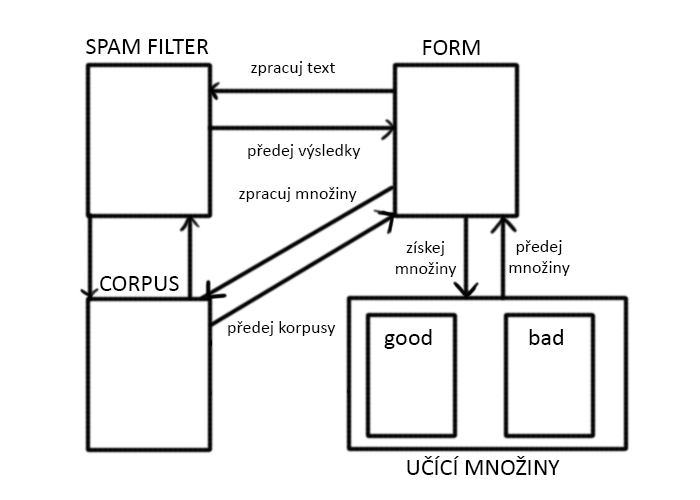
\includegraphics[width=\textwidth]{grafPredavani.png}
\end{figure}

\section{Corpus}
\textbf{\textit{Corpus.cs}} je třída, která vytváří korpusy s tokeny - slovy a jejich četnostmi. Jako taková obsahuje funkce pro zpracování textu z text readeru, vytvoření setříděného slovníku tokenů a přidánim jejich četnosti v daném korpusu.

\section{Spam filter}
Třída \textbf{\textit{SpamFilter.cs}} je nejdůležitější třídou celého řešení. Obsahuje metody pro zpracování testovacích množin, výpočet pravděpodobností tokenů a nakonec výpočet pravděpodobnosti toho, zda je text spam. v této sekci si dále popíšeme nejdůležitější části třídy \textbf{\textit{SpamFilter.cs}}

\subsection{ListAtributu}
\textbf{\textit{ListAtributu}} je vnitřní třídou třídy \textbf{\textit{SpamFilter.cs}} obsahující důležité atributy pro spam filter podle Grahama. Mezi tyto atributy patří:
\begin{itemize}
\item
VahaDobrehoTokenu - násobek pro dobrý token, defaultně 2.
\item
MinTokenuProPridani - minimální počet výskytů tokenu ve spamu a hamu, aby se spočítala jeho pravděpodobnost, defaultně 5.
\item
MinSkore - minimální pravděpodobnost spamu, kterou může token mít (z toho důvodu, že i slova, která se běžně vyskytují jen v hamu můžou být součástí spamu), defaultně 0,011.
\item
MaxSkore - maximální pravděpodobnost spamu, kterou může token mít. Defaultně 0,99.
\item
PocetProJistySpam - počet výskytů tokenu ve spamu, aby se prohlásil za vždy spamové slovo, defaultně 10.
\item
PocetZajimavychSlov - počet zajímavých tokenů, které v testovaném textu zkoumáme. Defaultně 20 (podle článku Paula Grahama lze použít i 15 slov pro dosažení vysoké přesnosti).
\end{itemize}

\subsection{SpoctiPravdepodobostTokenu}
Jedná se o funkci implementující Grahamův algoritmus (obr. 3.2). Algoritmus obsahuje následující proměnné:

\begin{itemize}
\item
d - počet výskytů tokenu v hamu
\item
s - počet výskytů tokenu ve spamu
\item
dobryfaktor - faktor spočítaný vzorcem $min(1, d / pocetHamTokenu)$
\item
spatnyfaktor - faktor spočítaný vzorcem $min(1, s / pocetSpamTokenu)$
\end{itemize}

z těchto proměnných se následně vypočítá pravděpodobnost tokenu přes vzorec:

\begin{center}
$max(MinSkore, min(MaxSkore, \frac{spatnyfaktor}{dobryfaktor + spatnyfaktor}))$
\end{center}

pokud se token vyskytuje pouze ve spamu (hodnota d je 0) tak se nastaví jeho pravděpodobnost na 0.9998 nebo 0.9999 pokud se vyskytuje ve spamu alespoň 10-krát.

\begin{figure}[!ht]
  \centering
    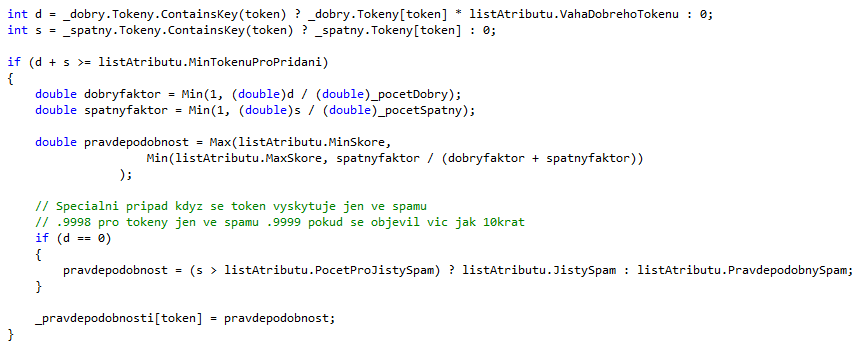
\includegraphics[width=\textwidth]{grahamAlgorithm.png}
    \caption{Grahamův algoritmus}
\end{figure}

\subsection{Test}
funkce Test zjišťuje pravděpodobnost toho, zda je spam či ne podle 20 "nejzajímavějších" slov - 20 tokenů, které mají pravděpodobnost nejblíže k 0 či 1. Funkce implementuje naivní Bayesovský klasifikátor (obr 3.3) a obsahuje proměnné:

\begin{itemize}
\item
nasob - součin všech pravděpodobností, že token je spam
\item
komb - součin všech pravděpodobností, že token není spam
\item
pravdepodobnosti - pole pravděpodobností nejzajímavějších slov textu
\end{itemize}

pomocí těchto proměnných se nakonec vypočítá pravděpodobnost, že text je spam přes vzorec $\frac{nasob}{nasob + komb}$

\begin{figure}[!ht]
  \centering
    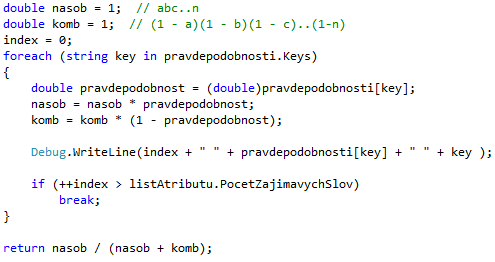
\includegraphics[width=\textwidth]{naiveBayes.png}
    \caption{Algoritmus naivního Bayesovského klasifikátoru}
\end{figure}

\subsection{Form - GUI}

obsluha GUI (viz. obr.3.4) je velice snadná. dá se popsat v několika krocích:

\begin{itemize}
\item
Stiskněte tlačítko \textit{"Načti testovací data"} pro načtení korpusů s hamem a spamem
\item
Můžete testovat předem připravené zprávy (stisknutím jednoho z tlačítek \textit{"Testovací zpráva"}) nebo napsáním vlastního textu do text boxu zadáte vlastní text pro testování. Po zadání textu jen stisknete tlačítko \textit{"Test Box Text"} a počkáte na vyhodnocení (zobrazí se jako zpráva \textit{"score: pravděpodobnost"} na první řádce text boxu)
\item
Pro výpis pravděpodobností do souboru \textit{out.txt} stačí stisknout tlačítko \textit{".ToFile()"}
\item
Pro načtení pravděpodobností ze souboru \textit{out.txt} stačí stisknout tlačítko \textit{".FromFile()"}
\end{itemize}

\begin{figure}[!ht]
  \centering
    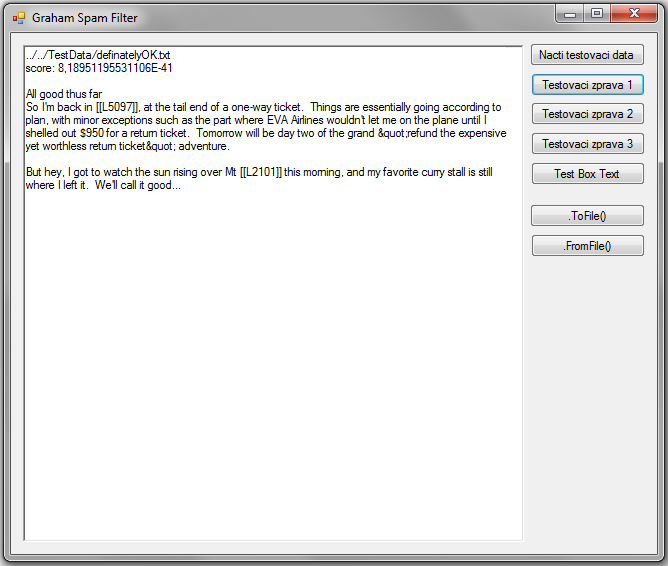
\includegraphics[width=\textwidth]{gui.png}
    \caption{Grafické uživatelské rozhraní}
\end{figure}

\chapter{Závěr}
Problém filtrování spamu mi přišel velmi zajímavý. Přístup Paula Grahama jsem si zvolil z důvodu, že přestože se jedná o celkem snadno implementovatelný algoritmus, je překvapivě přesný. Přibližně 99,5\% zpráv se určí správně jako spamové zprávy a pouze 0,03\% z nich jsou "false positive" - tedy nespamové e-mail vyhodnocené jako spam při dostatečně velké učící množině. Moje implementace má nižší přesnost, a to z důvodu velikosti korpusů. Ve svých textech Paul Graham uvádí, že používá až několik tisíc e-mailů pro dobré i špatné testovací množiny zatímco moje implementace používá pouze několik stovek. Přesto takovéto množství by mělo mít přesnost vyšší než 90\%.

Řešení bylo testováno pouze na anglicky psaných e-mailech vzhledem k jejich snadnější dostupnosti.

\bibliographystyle{csplainnat}
\bibliography{semestralka}
\end{document}
